% This is a default-selection of plugins that are used widely in this repo.

\documentclass[a4paper,10pt,fleqn]{article}
\usepackage[utf8]{inputenc}

% deutsche Trennmuster etc.
\usepackage[ngerman]{babel}
\usepackage[T1]{fontenc}

% mathematical simbols and fonts
\usepackage{mathtools} 
\usepackage{amssymb}
\usepackage{amsmath}
\usepackage{ntheorem}
\usepackage{polynom}
\usepackage{marvosym}
\usepackage{tabu}
\renewcommand*{\bmod}{\mathbin{\%}}
\everymath{\displaystyle}

\usepackage{multicol}
\usepackage{color}
\usepackage[usenames,dvipsnames]{xcolor}
\setlength{\columnsep}{1cm}
\setlength{\columnseprule}{0.25pt}
\def\columnseprulecolor{\color{gray}}
\usepackage{hyperref}

\usepackage[margin=1.5cm]{geometry}
\usepackage{graphicx}
\usepackage{pgfplots}
\pgfplotsset{compat=1.10}

%Code higlighting

\usepackage{minted}

% make lists more compact:
\newlength{\wideitemsep}
\setlength{\wideitemsep}{.5\itemsep}
\addtolength{\wideitemsep}{-5pt}
\let\olditem\item
\renewcommand{\item}{\setlength{\itemsep}{\wideitemsep}\olditem}
\renewcommand{\arraystretch}{1.25}

\title{Zusammenfassung AD1}
\author{Fabian Hauser}
 
\begin{document}
\maketitle


Software soll, \emph{Robust}, \emph{Adaptierbar} und \emph{Wiederverwendbar} sein, was via \emph{Abstraktion}, \emph{Kapselung} und \emph{Modularität} erreicht werden soll.

\section{Datenstrukturen}
\subsection{Arrays}

Arrays sind Container-Objekte, und enthalten im Java immer nur Referenzen auf gleichartige Objekte.

\paragraph{Vorteile}
\begin{itemize}
	\item Schneller Random Access (immer gleich lang)
\end{itemize}

\paragraph{Nachteile}
\begin{itemize}
	\item Kann nicht einfach vergrössert werden (umkopieren nötig)
	\item Einfügen, Löschen \& Sortieren aufwändig.
\end{itemize}

\subsection{LinkedList}

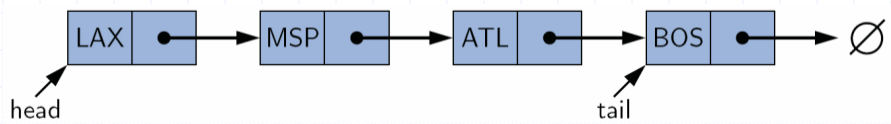
\includegraphics[scale=0.3]{img/linkedlist.png} \\
Nutzt Rekursion (Referenz auf eigenen Typen) zum feststellen des jeweilig nächsten Elements

\paragraph{Vorteile}
\begin{itemize}
	\item Entfernen eines Knotens immer gleich (einfach)
	\item Einfügen eines Knotens immer gleich (einfach)
\end{itemize}

\paragraph{Nachteile}
\begin{itemize}
	\item Random Access braucht lange (iterieren durch alle Elemente)
	\item Nicht Thread-sicher (\emph{Collections.synchronizedList(new LinkedList(...))})
\end{itemize}

\subsubsection{Doubly-Linked-List}

Es wird jeweils auch das Previous-Element referenziert; Vorteil: es können Elemente von beiden Enden schnell abgeholt werden.

\subsubsection{Circularly-Linked-Lists}

Zirkuläre Listen, d.h., das letzte Element ist mit dem ersten verknüpft. es gibt jeweils einen Cursor auf das aktuelle Element.

for(int[] currencyUnit : currencyUnits)   


\subsection{Pseudocode}
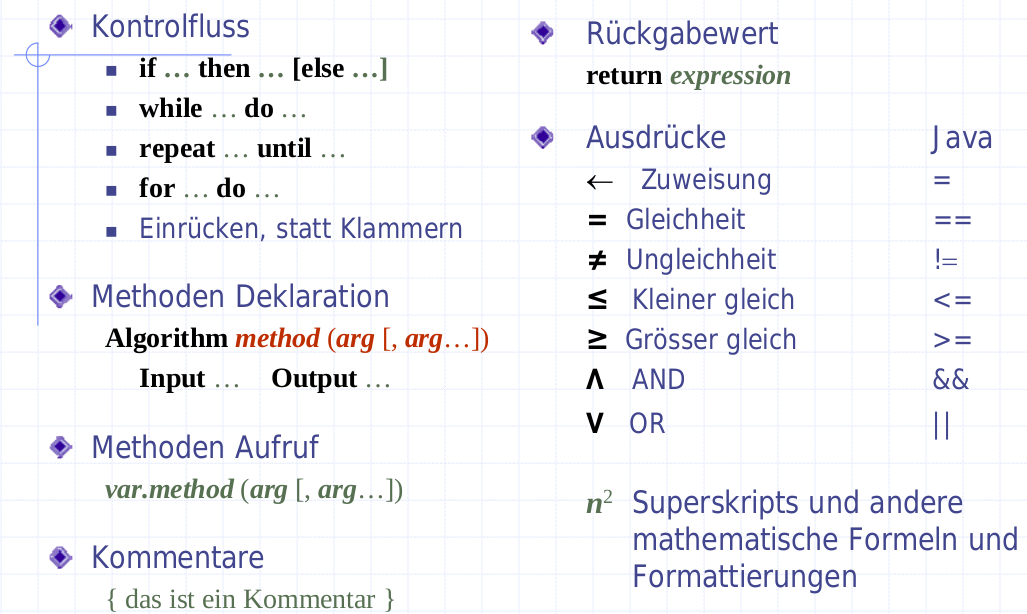
\includegraphics[scale=0.3]{img/pseudocode.png}

\subsection{Laufzeitverhalten}

\subsubsection{Zeitliche Funktionen}
\begin{itemize}
	\item konstant $\approx 1$
	\item logarithmisch $\approx \log n$
	\item linear $\approx  n$
	\item N-Log-N $\approx n \log n$
	\item quadratisch $\approx n^2$
	\item qubisch $\approx n^3$
	\item exponentiell $\approx 2^n$
\end{itemize}

\subsubsection{Big-Oh Notation}
 
Berechnung der Präfixe: Herausfinden, wie oft eine Operation in einem Algorithmus durchläuft; dabei ist nur essentiell, ob $n$, $n^2$ etc. Durchläufe stattgefunden haben.

Beispiel: $O(n^2)$

\subsubsection{Big-Omega, Big-Theta}

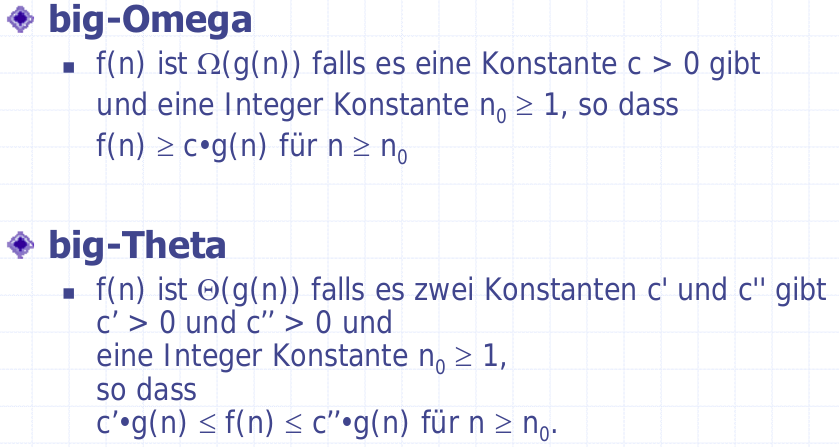
\includegraphics[scale=0.3]{img/verwandte-big-oh.png}

\subsubsection{Vergleich Big-Oh, Omega, Theta}

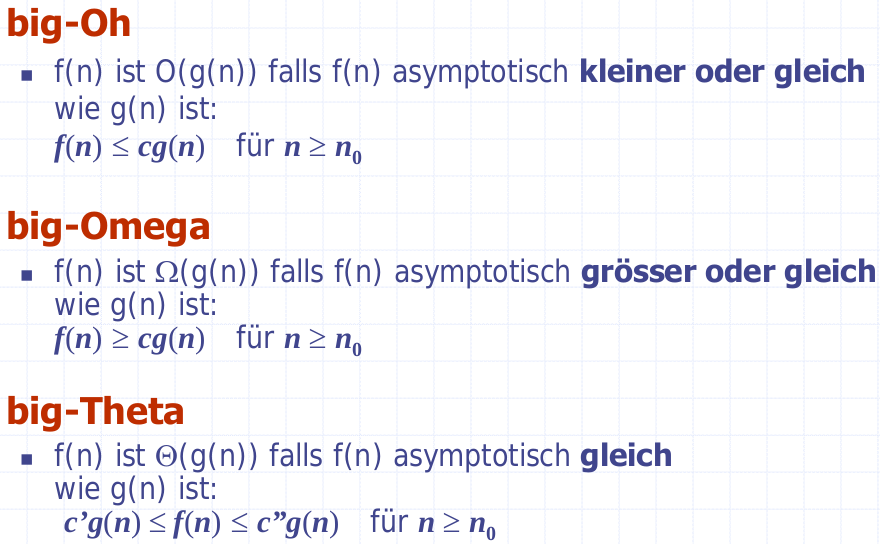
\includegraphics[scale=0.3]{img/big-oh-vergleich.png}

\subsection{Rekursion}

Braucht:
\begin{itemize}
	\item Verankerung / base case(s): Ende des Rekursiven Aufrufes / Abbruchbedingung
	\item Methode ruft sich selber auf, bringt den Zustand näher an die Verankerung.
\end{itemize}

\subsubsection{Lineare Rekursion}

\subsubsection{Binäre Rekursion}

\subsubsection{Andere Rekursion}



\section{Patternator}

\subsection{Adapter}
\subsubsection{Objectadapter}

Besser für Sicherheit

Implementation via Klassenvariable

\subsubsection{Classadapter}

Einfacher/Flexibel

Implementation Interface

\subsection{Datenstrukturen}

\subsubsection{Stack}

Bei fixem Stack, Performance $O(n)$ Speicherplatzbedarf und $O(1)$ Zugriffsgeschwindigkeit.

\subsubsection{Dequeue}

LIFO

\subsubsection{Queue}

\paragraph{Ringbuffer} (Zyklische Queue), Ansatz: Array oder Node-Basiert (Linked List)

\paragraph{Double-Ended-Queue (DeQueue/Deque)} kann von beiden Seiten durchlaufen werden.

\subsubsection{Lists}

Mittleres verhalten: T(n)/n


\subsubsection{Trees}

Höhe: $\sqrt(\text{nodes})$


\paragraph{Binary Tree}

Hat immer zwei Kindknoten

Durchiterieren:
\begin{description}
	\item[Preorder Traversierung] \hfill \\
		Es wird jeweils vom Root links durch die Kinder durchgegangen
	\item[Postorder Traversierung] \hfill \\
		Es wird vom linksten Leaf den leafs von links her durchgegangen.
	\item[Breadth-First]\hfill \\
		Es werden immer alle Knoten von links nach rechts der Ebene nach abgegangen, beginnend mit dem root
	\item[Inorder Traversierung] \hfill \\
		Es wird immer zuerst beim linksuntersten element begonnen, und so dem tree entlang weiter verfahren.
	\item[Euler Tour Traveriserung] \hfill \\
		Generischer Fall (Preorder, Postorder und Inorder durchgang).
\end{description}

\subsection{Iterators}

Pointer zeigt zwischen Elemente

\subsection{Information Tree}



\section{Java cheats}
\subsection{Arrays}
\begin{description}
	
	\item[Fast array copy] \hfill \\
		public static void arraycopy(Object src, int srcPos, Object dest, int destPos, int length)

\end{description}
\end{document}